% !TeX encoding = UTF-8
% !TeX root = sigmod2018.tex
% !TeX spellcheck = en_US

\section{End-to-End Evaluation}
\label{sec:SSBEval}

\begin{figure*}[t!]%
	\centering
	\footnotesize
	\graphicspath{{results/ssb/report/}}
	\begin{subfigure}[t]{6.5in}
		% GNUPLOT: LaTeX picture with Postscript
\begingroup
  \makeatletter
  \providecommand\color[2][]{%
    \GenericError{(gnuplot) \space\space\space\@spaces}{%
      Package color not loaded in conjunction with
      terminal option `colourtext'%
    }{See the gnuplot documentation for explanation.%
    }{Either use 'blacktext' in gnuplot or load the package
      color.sty in LaTeX.}%
    \renewcommand\color[2][]{}%
  }%
  \providecommand\includegraphics[2][]{%
    \GenericError{(gnuplot) \space\space\space\@spaces}{%
      Package graphicx or graphics not loaded%
    }{See the gnuplot documentation for explanation.%
    }{The gnuplot epslatex terminal needs graphicx.sty or graphics.sty.}%
    \renewcommand\includegraphics[2][]{}%
  }%
  \providecommand\rotatebox[2]{#2}%
  \@ifundefined{ifGPcolor}{%
    \newif\ifGPcolor
    \GPcolortrue
  }{}%
  \@ifundefined{ifGPblacktext}{%
    \newif\ifGPblacktext
    \GPblacktexttrue
  }{}%
  % define a \g@addto@macro without @ in the name:
  \let\gplgaddtomacro\g@addto@macro
  % define empty templates for all commands taking text:
  \gdef\gplbacktext{}%
  \gdef\gplfronttext{}%
  \makeatother
  \ifGPblacktext
    % no textcolor at all
    \def\colorrgb#1{}%
    \def\colorgray#1{}%
  \else
    % gray or color?
    \ifGPcolor
      \def\colorrgb#1{\color[rgb]{#1}}%
      \def\colorgray#1{\color[gray]{#1}}%
      \expandafter\def\csname LTw\endcsname{\color{white}}%
      \expandafter\def\csname LTb\endcsname{\color{black}}%
      \expandafter\def\csname LTa\endcsname{\color{black}}%
      \expandafter\def\csname LT0\endcsname{\color[rgb]{1,0,0}}%
      \expandafter\def\csname LT1\endcsname{\color[rgb]{0,1,0}}%
      \expandafter\def\csname LT2\endcsname{\color[rgb]{0,0,1}}%
      \expandafter\def\csname LT3\endcsname{\color[rgb]{1,0,1}}%
      \expandafter\def\csname LT4\endcsname{\color[rgb]{0,1,1}}%
      \expandafter\def\csname LT5\endcsname{\color[rgb]{1,1,0}}%
      \expandafter\def\csname LT6\endcsname{\color[rgb]{0,0,0}}%
      \expandafter\def\csname LT7\endcsname{\color[rgb]{1,0.3,0}}%
      \expandafter\def\csname LT8\endcsname{\color[rgb]{0.5,0.5,0.5}}%
    \else
      % gray
      \def\colorrgb#1{\color{black}}%
      \def\colorgray#1{\color[gray]{#1}}%
      \expandafter\def\csname LTw\endcsname{\color{white}}%
      \expandafter\def\csname LTb\endcsname{\color{black}}%
      \expandafter\def\csname LTa\endcsname{\color{black}}%
      \expandafter\def\csname LT0\endcsname{\color{black}}%
      \expandafter\def\csname LT1\endcsname{\color{black}}%
      \expandafter\def\csname LT2\endcsname{\color{black}}%
      \expandafter\def\csname LT3\endcsname{\color{black}}%
      \expandafter\def\csname LT4\endcsname{\color{black}}%
      \expandafter\def\csname LT5\endcsname{\color{black}}%
      \expandafter\def\csname LT6\endcsname{\color{black}}%
      \expandafter\def\csname LT7\endcsname{\color{black}}%
      \expandafter\def\csname LT8\endcsname{\color{black}}%
    \fi
  \fi
    \setlength{\unitlength}{0.0500bp}%
    \ifx\gptboxheight\undefined%
      \newlength{\gptboxheight}%
      \newlength{\gptboxwidth}%
      \newsavebox{\gptboxtext}%
    \fi%
    \setlength{\fboxrule}{0.5pt}%
    \setlength{\fboxsep}{1pt}%
\begin{picture}(9360.00,1440.00)%
    \gplgaddtomacro\gplbacktext{%
      \csname LTb\endcsname%
      \put(412,297){\makebox(0,0)[r]{\strut{}$0$}}%
      \csname LTb\endcsname%
      \put(412,500){\makebox(0,0)[r]{\strut{}$0.5$}}%
      \csname LTb\endcsname%
      \put(412,703){\makebox(0,0)[r]{\strut{}$1$}}%
      \csname LTb\endcsname%
      \put(412,905){\makebox(0,0)[r]{\strut{}$1.5$}}%
      \csname LTb\endcsname%
      \put(412,1108){\makebox(0,0)[r]{\strut{}$2$}}%
      \csname LTb\endcsname%
      \put(412,1311){\makebox(0,0)[r]{\strut{}$2.5$}}%
      \csname LTb\endcsname%
      \put(1052,124){\makebox(0,0){\strut{}Q1.1}}%
      \csname LTb\endcsname%
      \put(1579,124){\makebox(0,0){\strut{}Q1.2}}%
      \csname LTb\endcsname%
      \put(2106,124){\makebox(0,0){\strut{}Q1.3}}%
      \csname LTb\endcsname%
      \put(2633,124){\makebox(0,0){\strut{}Q2.1}}%
      \csname LTb\endcsname%
      \put(3160,124){\makebox(0,0){\strut{}Q2.2}}%
      \csname LTb\endcsname%
      \put(3687,124){\makebox(0,0){\strut{}Q2.3}}%
      \csname LTb\endcsname%
      \put(4214,124){\makebox(0,0){\strut{}Q3.1}}%
      \csname LTb\endcsname%
      \put(4740,124){\makebox(0,0){\strut{}Q3.2}}%
      \csname LTb\endcsname%
      \put(5267,124){\makebox(0,0){\strut{}Q3.3}}%
      \csname LTb\endcsname%
      \put(5794,124){\makebox(0,0){\strut{}Q3.4}}%
      \csname LTb\endcsname%
      \put(6321,124){\makebox(0,0){\strut{}Q4.1}}%
      \csname LTb\endcsname%
      \put(6848,124){\makebox(0,0){\strut{}Q4.2}}%
      \csname LTb\endcsname%
      \put(7375,124){\makebox(0,0){\strut{}Q4.3}}%
    }%
    \gplgaddtomacro\gplfronttext{%
      \csname LTb\endcsname%
      \put(94,804){\rotatebox{-270}{\makebox(0,0){\strut{}Relative Runtime}}}%
      \csname LTb\endcsname%
      \put(8990,1174){\makebox(0,0)[r]{\strut{}Unprotected}}%
      \csname LTb\endcsname%
      \put(8990,1026){\makebox(0,0)[r]{\strut{}DMR}}%
      \csname LTb\endcsname%
      \put(8990,878){\makebox(0,0)[r]{\strut{}Early}}%
      \csname LTb\endcsname%
      \put(8990,730){\makebox(0,0)[r]{\strut{}Late}}%
      \csname LTb\endcsname%
      \put(8990,582){\makebox(0,0)[r]{\strut{}Continuous}}%
      \csname LTb\endcsname%
      \put(8990,434){\makebox(0,0)[r]{\strut{}Reencoding}}%
    }%
    \gplbacktext
    \put(0,0){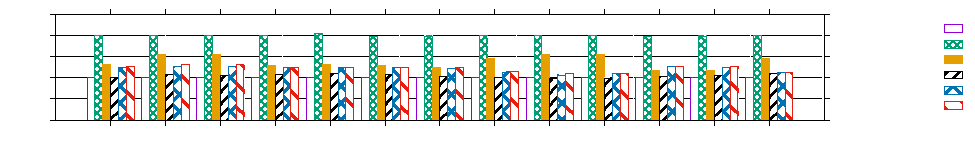
\includegraphics{norm-all_SSE}}%
    \gplfronttext
  \end{picture}%
\endgroup

	\end{subfigure}
	\vspace{-0.3cm}
	\caption{Relative SSB runtimes for vectorized (SSE4.2) execution (average over all scale factors).}%
	\label{fig:eval:runtime}%
	\vspace{-0.4cm}
\end{figure*}

We evaluate our \emph{AHEAD} approach using the analytical SSB benchmark~\cite{oneil2009ssbm}. All experiments are conducted without error induction, because the conditional SDC probabilities are known (cf. Section~\ref{sec:DataHardening}). Our system was equipped with one Intel\textsuperscript{\textregistered} Core\textsuperscript{\texttrademark} i7 6820HK CPU (\textat 2.70GHz), and 16 GB of DDR3 main memory (\textat 2133MHz) running 64\=bit Ubuntu 16.04.3 LTS using GCC 7.1.0.





\subsection{Implementation}
\label{sec:Implementation}
We implemented a self\=contained \emph{AHEAD} prototype using a column\=at\=a\=time execution model\footnote{The prototype is available on GitHub \url{https://brics-db.github.io/}, see Appendix~\ref{sec:GitHub}}, due to the following: (1) We wanted to have both protected and unprotected data to measure the appropriate runtimes in a uniform way. This requires to have operators for both available simultaneously, which would require to reimplement all physical operators in an existing DBMS. (2) We want to first show that our approach is feasible, without any side effects, so that it can then be integrated in an existing system. Our \emph{AHEAD} prototype is completely written in C++ using well-known column store concepts~\cite{DBLP:journals/ftdb/AbadiBHIM13} and supports both unprotected and hardened query processing in a unified way for comparability. For that, a separate type system allows to distinguish data types and the actual width of a type is adjusted through a mere \texttt{typedef}. Our current prototype differentiates between 8-, 16-, 32-, and 64\=bit data types, i.e. we do byte-level compression on native CPU register granularity. We call the types \texttt{tinyint}, \texttt{shortint}, \texttt{int}, and \texttt{bigint}, respectively. The hardened variants (\texttt{restiny}, \texttt{resshort}, \texttt{resint}, and \texttt{resbig}, respectively) are mapped to the next available native integer width, i.e. 16, 32, 64, and again 64 bits. For \texttt{tinyint}, this allows \(A\)s up to a width of 8\=bits, for the others \(A\)s up to 16\=bit and \texttt{bigint} is limited to 48\=bits of actual data\footnote{128-bit integer implementations like the Boost C++ library could be used to support larger integer widths, using a simple \texttt{typedef} change for scalar code.}. For strings, we use a separate data heap and the data column contains pointers to the actual string values. Our current implementation does not use dictionary compression. The physical query operators support all these data types through template programming to ease the data type specialization. Furthermore, for the vectorized operators, the template programming helps to specialize only those details of the SSE operators which require calls to specific intrinsics. For instance, the algorithm skeletons are the same for all integer types, but e.g. multiplication requires different intrinsics for 16\=bit (\texttt{\_mm\_mullo\_epi16}, \texttt{pmullw}) or 32\=bit (\texttt{\_mm\_mullo\_epi32}, \texttt{pmulld}) data, just to name two examples. We implemented both, scalar and SSE4.2 query operators, while Hash\=join and Group\=by use Google's \texttt{dense\_hash\_map}\footnote{\url{https://github.com/sparsehash}} for performance reasons. All of the $13$ SSB queries are manually written, guided by the query explanation output from MonetDB~\cite{boncz2002monet}. We chose single\=threaded execution to avoid any side\=effects and to precisely measure the overhead.





\subsection{SSB Runtime Performance}
We compare our \emph{AHEAD} approach with the \emph{Unprotected} baseline and dual modular redundancy (DMR). In the \emph{Unprotected} baseline, data is always compressed on a byte-level based on the column characteristics. \emph{DMR} uses the \emph{Unprotected} setting and replicates all data in main memory, executes each query twice sequentially, and afterwards a voter compares both results. Our \emph{AHEAD} approach hardens each column using the largest currently known \(A\) for the corresponding column data width from Table~\ref{tab:optimalAs}. Thus, compared to \emph{Unprotected} setting, \emph{AHEAD} increases the data width of each column to the next byte level. For all approaches, we measured all 13 SSB queries for scalar and vectorized (SSE4.2) execution and we varied the SSB scale factor from 1 to 10. Each single experiment ran 10 times. Figure~\ref{fig:eval:runtime} shows vectorized (SSE4.2) runtimes relative to the \emph{Unprotected} baseline. \emph{DMR} results in the expected runtime overhead of about 100\%, because each query is executed twice. For our \emph{AHEAD} detection schemes, we can draw the following conclusions:

\textbf{Early Detection} has a very high initial overhead of the \(\Delta\) operator leading to an overhead between 64\% and 185\% for scalar execution (cf. Figure~\ref{fig:eval:runtime:scalar} in Appendix~\ref{sec:SSBEval:scalar}). With vectorization, early detection is much faster, because \(\Delta\) benefits so much more than the other operators, and the overhead is reduced to 18\% to 56\%.

\textbf{Late Detection} executes \(\Delta\) only on hardened data arrays prior to the aggregation or grouping and newly created intermediates like IDs are never hardened. Consequently, it checks much less values and errors are detected only very late in the query, resulting in overheads of at most 10\% for both scalar and SSE4.2 execution. Errors might add up to valid code words, so that less are detected.

\textbf{Continuous and Reencoding} use the same query plan as the baseline but with AN\=coding\=aware operators, where the latter reencode each operator's output. As we assume no particular error rate or bit flip weight distribution, our policy for the new \(A\) for \emph{Reencoding} is to decrease the bit width of \(A\) by $1$ for each input. For that, we use an extended version of Table~\ref{tab:optimalAs}. This is meant to simply show the feasibility of reencoding each operator output. The runtime of \emph{Continuous Detection} lies between Early and Late with about 10\% to 26\% (scalar) and 7\% to 28\% (vectorized) overhead. This is due to the tight integration of error detection in each operator. \emph{Reencoding} adds virtually no overhead to \emph{Continuous} with overheads of 10\% to 27\% (scalar) and 10\% to 31\% (SSE4.2).

\begin{figure}%
	\footnotesize
	\graphicspath{{results/ssb/}}
	\input{results/ssb/scalarVSvector}%
	\vspace{-1.5em}
	\caption{Scalar against vectorized runtimes (SSB 1.1 to 1.3).}%
	\label{fig:vectorVSscalar}%
	\vspace{-0.4cm}
\end{figure}





\subsection{Scalar vs. Vectorized Execution}
Having compared the detection variants per query, we now show in more detail the impact of the vectorization. We use the average over SSB queries 1.1 to 1.3 because they filter on small integer data and there the impact of vectorization is greatest. Vectorized \emph{Unprotected} serves as baseline. Figure~\ref{fig:vectorVSscalar} shows that all variants benefit greatly from SSE4.2 vectorization for queries 1.1 to 1.3. The speedup factor is shown at the arrows for each variant, as well. For \emph{Early} it is larger because \(\Delta\) benefits very much. Note that the speedups for \emph{Continous} and \emph{Reencode} are only slightly smaller than for \emph{Unprotected}, although they operate on half as many code words per SIMD instruction. Consequently, our AHEAD approach scales well using vectorization.

\begin{figure}%
	\footnotesize
	\graphicspath{{results/ssb/}}
	\null
	\begin{subfigure}{1.4in}
		% GNUPLOT: LaTeX picture with Postscript
\begingroup
  \makeatletter
  \providecommand\color[2][]{%
    \GenericError{(gnuplot) \space\space\space\@spaces}{%
      Package color not loaded in conjunction with
      terminal option `colourtext'%
    }{See the gnuplot documentation for explanation.%
    }{Either use 'blacktext' in gnuplot or load the package
      color.sty in LaTeX.}%
    \renewcommand\color[2][]{}%
  }%
  \providecommand\includegraphics[2][]{%
    \GenericError{(gnuplot) \space\space\space\@spaces}{%
      Package graphicx or graphics not loaded%
    }{See the gnuplot documentation for explanation.%
    }{The gnuplot epslatex terminal needs graphicx.sty or graphics.sty.}%
    \renewcommand\includegraphics[2][]{}%
  }%
  \providecommand\rotatebox[2]{#2}%
  \@ifundefined{ifGPcolor}{%
    \newif\ifGPcolor
    \GPcolortrue
  }{}%
  \@ifundefined{ifGPblacktext}{%
    \newif\ifGPblacktext
    \GPblacktexttrue
  }{}%
  % define a \g@addto@macro without @ in the name:
  \let\gplgaddtomacro\g@addto@macro
  % define empty templates for all commands taking text:
  \gdef\gplbacktext{}%
  \gdef\gplfronttext{}%
  \makeatother
  \ifGPblacktext
    % no textcolor at all
    \def\colorrgb#1{}%
    \def\colorgray#1{}%
  \else
    % gray or color?
    \ifGPcolor
      \def\colorrgb#1{\color[rgb]{#1}}%
      \def\colorgray#1{\color[gray]{#1}}%
      \expandafter\def\csname LTw\endcsname{\color{white}}%
      \expandafter\def\csname LTb\endcsname{\color{black}}%
      \expandafter\def\csname LTa\endcsname{\color{black}}%
      \expandafter\def\csname LT0\endcsname{\color[rgb]{1,0,0}}%
      \expandafter\def\csname LT1\endcsname{\color[rgb]{0,1,0}}%
      \expandafter\def\csname LT2\endcsname{\color[rgb]{0,0,1}}%
      \expandafter\def\csname LT3\endcsname{\color[rgb]{1,0,1}}%
      \expandafter\def\csname LT4\endcsname{\color[rgb]{0,1,1}}%
      \expandafter\def\csname LT5\endcsname{\color[rgb]{1,1,0}}%
      \expandafter\def\csname LT6\endcsname{\color[rgb]{0,0,0}}%
      \expandafter\def\csname LT7\endcsname{\color[rgb]{1,0.3,0}}%
      \expandafter\def\csname LT8\endcsname{\color[rgb]{0.5,0.5,0.5}}%
    \else
      % gray
      \def\colorrgb#1{\color{black}}%
      \def\colorgray#1{\color[gray]{#1}}%
      \expandafter\def\csname LTw\endcsname{\color{white}}%
      \expandafter\def\csname LTb\endcsname{\color{black}}%
      \expandafter\def\csname LTa\endcsname{\color{black}}%
      \expandafter\def\csname LT0\endcsname{\color{black}}%
      \expandafter\def\csname LT1\endcsname{\color{black}}%
      \expandafter\def\csname LT2\endcsname{\color{black}}%
      \expandafter\def\csname LT3\endcsname{\color{black}}%
      \expandafter\def\csname LT4\endcsname{\color{black}}%
      \expandafter\def\csname LT5\endcsname{\color{black}}%
      \expandafter\def\csname LT6\endcsname{\color{black}}%
      \expandafter\def\csname LT7\endcsname{\color{black}}%
      \expandafter\def\csname LT8\endcsname{\color{black}}%
    \fi
  \fi
    \setlength{\unitlength}{0.0500bp}%
    \ifx\gptboxheight\undefined%
      \newlength{\gptboxheight}%
      \newlength{\gptboxwidth}%
      \newsavebox{\gptboxtext}%
    \fi%
    \setlength{\fboxrule}{0.5pt}%
    \setlength{\fboxsep}{1pt}%
\begin{picture}(2000.00,1440.00)%
    \gplgaddtomacro\gplbacktext{%
      \csname LTb\endcsname%
      \put(380,421){\makebox(0,0)[r]{\strut{}$0$}}%
      \csname LTb\endcsname%
      \put(380,561){\makebox(0,0)[r]{\strut{}$0.2$}}%
      \csname LTb\endcsname%
      \put(380,701){\makebox(0,0)[r]{\strut{}$0.4$}}%
      \csname LTb\endcsname%
      \put(380,841){\makebox(0,0)[r]{\strut{}$0.6$}}%
      \csname LTb\endcsname%
      \put(380,982){\makebox(0,0)[r]{\strut{}$0.8$}}%
      \csname LTb\endcsname%
      \put(380,1122){\makebox(0,0)[r]{\strut{}$1$}}%
      \csname LTb\endcsname%
      \put(380,1262){\makebox(0,0)[r]{\strut{}$1.2$}}%
      \csname LTb\endcsname%
      \put(380,1402){\makebox(0,0)[r]{\strut{}$1.4$}}%
      \csname LTb\endcsname%
      \put(794,248){\makebox(0,0){\strut{}1}}%
      \csname LTb\endcsname%
      \put(1095,248){\makebox(0,0){\strut{}2}}%
      \csname LTb\endcsname%
      \put(1397,248){\makebox(0,0){\strut{}3}}%
      \csname LTb\endcsname%
      \put(1698,248){\makebox(0,0){\strut{}4$^*$}}%
    }%
    \gplgaddtomacro\gplfronttext{%
      \csname LTb\endcsname%
      \put(94,787){\rotatebox{-270}{\makebox(0,0){\strut{}Relative Runtime}}}%
      \csname LTb\endcsname%
      \put(941,111){\makebox(0,0)[r]{\strut{}Scalar}}%
      \csname LTb\endcsname%
      \put(1630,111){\makebox(0,0)[r]{\strut{}SSE4.2}}%
    }%
    \gplbacktext
    \put(0,0){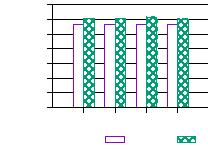
\includegraphics{minbfw_runtime}}%
    \gplfronttext
  \end{picture}%
\endgroup
%
		\vspace{-0.5em}
		\caption{Runtime}
		\label{fig:minbfw:runtime}
	\end{subfigure}
	\hfill
	\begin{subfigure}{1.7in}
		% GNUPLOT: LaTeX picture with Postscript
\begingroup
  \makeatletter
  \providecommand\color[2][]{%
    \GenericError{(gnuplot) \space\space\space\@spaces}{%
      Package color not loaded in conjunction with
      terminal option `colourtext'%
    }{See the gnuplot documentation for explanation.%
    }{Either use 'blacktext' in gnuplot or load the package
      color.sty in LaTeX.}%
    \renewcommand\color[2][]{}%
  }%
  \providecommand\includegraphics[2][]{%
    \GenericError{(gnuplot) \space\space\space\@spaces}{%
      Package graphicx or graphics not loaded%
    }{See the gnuplot documentation for explanation.%
    }{The gnuplot epslatex terminal needs graphicx.sty or graphics.sty.}%
    \renewcommand\includegraphics[2][]{}%
  }%
  \providecommand\rotatebox[2]{#2}%
  \@ifundefined{ifGPcolor}{%
    \newif\ifGPcolor
    \GPcolortrue
  }{}%
  \@ifundefined{ifGPblacktext}{%
    \newif\ifGPblacktext
    \GPblacktexttrue
  }{}%
  % define a \g@addto@macro without @ in the name:
  \let\gplgaddtomacro\g@addto@macro
  % define empty templates for all commands taking text:
  \gdef\gplbacktext{}%
  \gdef\gplfronttext{}%
  \makeatother
  \ifGPblacktext
    % no textcolor at all
    \def\colorrgb#1{}%
    \def\colorgray#1{}%
  \else
    % gray or color?
    \ifGPcolor
      \def\colorrgb#1{\color[rgb]{#1}}%
      \def\colorgray#1{\color[gray]{#1}}%
      \expandafter\def\csname LTw\endcsname{\color{white}}%
      \expandafter\def\csname LTb\endcsname{\color{black}}%
      \expandafter\def\csname LTa\endcsname{\color{black}}%
      \expandafter\def\csname LT0\endcsname{\color[rgb]{1,0,0}}%
      \expandafter\def\csname LT1\endcsname{\color[rgb]{0,1,0}}%
      \expandafter\def\csname LT2\endcsname{\color[rgb]{0,0,1}}%
      \expandafter\def\csname LT3\endcsname{\color[rgb]{1,0,1}}%
      \expandafter\def\csname LT4\endcsname{\color[rgb]{0,1,1}}%
      \expandafter\def\csname LT5\endcsname{\color[rgb]{1,1,0}}%
      \expandafter\def\csname LT6\endcsname{\color[rgb]{0,0,0}}%
      \expandafter\def\csname LT7\endcsname{\color[rgb]{1,0.3,0}}%
      \expandafter\def\csname LT8\endcsname{\color[rgb]{0.5,0.5,0.5}}%
    \else
      % gray
      \def\colorrgb#1{\color{black}}%
      \def\colorgray#1{\color[gray]{#1}}%
      \expandafter\def\csname LTw\endcsname{\color{white}}%
      \expandafter\def\csname LTb\endcsname{\color{black}}%
      \expandafter\def\csname LTa\endcsname{\color{black}}%
      \expandafter\def\csname LT0\endcsname{\color{black}}%
      \expandafter\def\csname LT1\endcsname{\color{black}}%
      \expandafter\def\csname LT2\endcsname{\color{black}}%
      \expandafter\def\csname LT3\endcsname{\color{black}}%
      \expandafter\def\csname LT4\endcsname{\color{black}}%
      \expandafter\def\csname LT5\endcsname{\color{black}}%
      \expandafter\def\csname LT6\endcsname{\color{black}}%
      \expandafter\def\csname LT7\endcsname{\color{black}}%
      \expandafter\def\csname LT8\endcsname{\color{black}}%
    \fi
  \fi
    \setlength{\unitlength}{0.0500bp}%
    \ifx\gptboxheight\undefined%
      \newlength{\gptboxheight}%
      \newlength{\gptboxwidth}%
      \newsavebox{\gptboxtext}%
    \fi%
    \setlength{\fboxrule}{0.5pt}%
    \setlength{\fboxsep}{1pt}%
\begin{picture}(2440.00,1440.00)%
    \gplgaddtomacro\gplbacktext{%
      \csname LTb\endcsname%
      \put(380,545){\makebox(0,0)[r]{\strut{}$0$}}%
      \csname LTb\endcsname%
      \put(380,716){\makebox(0,0)[r]{\strut{}$0.5$}}%
      \csname LTb\endcsname%
      \put(380,888){\makebox(0,0)[r]{\strut{}$1$}}%
      \csname LTb\endcsname%
      \put(380,1059){\makebox(0,0)[r]{\strut{}$1.5$}}%
      \csname LTb\endcsname%
      \put(380,1231){\makebox(0,0)[r]{\strut{}$2$}}%
      \csname LTb\endcsname%
      \put(380,1402){\makebox(0,0)[r]{\strut{}$2.5$}}%
      \csname LTb\endcsname%
      \put(882,372){\makebox(0,0){\strut{}1}}%
      \csname LTb\endcsname%
      \put(1271,372){\makebox(0,0){\strut{}2}}%
      \csname LTb\endcsname%
      \put(1661,372){\makebox(0,0){\strut{}3}}%
      \csname LTb\endcsname%
      \put(2050,372){\makebox(0,0){\strut{}4$^*$}}%
    }%
    \gplgaddtomacro\gplfronttext{%
      \csname LTb\endcsname%
      \put(94,725){\rotatebox{-270}{\makebox(0,0){\strut{}Relative Consumption}}}%
      \csname LTb\endcsname%
      \put(1161,235){\makebox(0,0)[r]{\strut{}Unprotected}}%
      \csname LTb\endcsname%
      \put(1161,111){\makebox(0,0)[r]{\strut{}Continuous}}%
      \csname LTb\endcsname%
      \put(2170,235){\makebox(0,0)[r]{\strut{}Bit-Packed}}%
      \csname LTb\endcsname%
      \put(1077,1128){\rotatebox{90}{\makebox(0,0)[l]{\strut{}1.43}}}%
      \csname LTb\endcsname%
      \put(1466,1128){\rotatebox{90}{\makebox(0,0)[l]{\strut{}1.49}}}%
      \csname LTb\endcsname%
      \put(1855,1128){\rotatebox{90}{\makebox(0,0)[l]{\strut{}1.55}}}%
      \csname LTb\endcsname%
      \put(2244,1128){\rotatebox{90}{\makebox(0,0)[l]{\strut{}1.61}}}%
    }%
    \gplbacktext
    \put(0,0){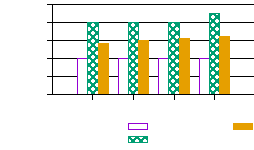
\includegraphics{minbfw_consumption}}%
    \gplfronttext
  \end{picture}%
\endgroup
%
		\vspace{-0.5em}
		\caption{Storage}
		\label{fig:minbfw:storage}
	\end{subfigure}
	\null
	\vspace{-1.5em}
	\caption{SSB query 1.1 runtime and storage comparison for \emph{Continuous} with different min bfw's (x axis). $4^*$: we increased \texttt{restiny} size to 32 bits to allow \(|A|>8\).}%
	\label{fig:minbfw}%
	\vspace{-0.5cm}
\end{figure}





\subsection{Influence of Bit Flip Weight}
Up to now, we used the largest \(A\) for data hardening in our experiments. We will now investigate the influence of different \(A\)s on the runtime and storage overhead of the \emph{Continuous} variant. For each hardened data type, we vary the \(A\) of all base and intermediate columns to the smallest one for guaranteed minimum bit flip weights (\emph{min bfw}) $1$ to $4$ from Table~\ref{tab:optimalAs}. We chose this scenario, because Kim et al.~\cite{DBLP:conf/isca/KimDKFLLWLM14} observed one to four bit flips in all newer DRAM modules. For the case of $4$, we let the \texttt{restiny} datatype be 32 bits wide to allow $|A|>8$. Due to our type system, this is a simple \texttt{typedef} change. Figure~\ref{fig:minbfw:runtime} shows the runtimes as in Figure~\ref{fig:eval:runtime}, while Figure~\ref{fig:minbfw:storage} shows the storage overhead. Runtimes differ only slightly for both scalar and SSE4.2 execution. With \emph{Continuous}, the storage consumption doubles for \emph{min bfw} $1$ to $3$, because we only work on native register widths. For \emph{min bfw} $4$, the storage overhead is slightly higher (126\%), since \texttt{restiny} is twice as big. This shows the limitation of our current byte-oriented compression. Willhalm et al. showed how to store data in a bit-packed fashion and how to evaluate even complex filter predicates in a vectorized manner~\cite{Willhalm:2009:SUF:1687627.1687671,willhalm2013vectorizing}. To overcome our current implementation limitation, we could use their approach. To show the benefit, we projected the storage consumption for \emph{bit-packed} compression in Figure~\ref{fig:minbfw:storage} as well, which displays potentials for reducing the memory overhead of our \emph{AHEAD} approach. Since bit-packing reduces the load on the memory subsystem, this \emph{might} improve query runtimes, too, but that remains to be seen.
